\documentclass[pdflatex,sn-basic,Numbered]{sn-jnl}

\usepackage{graphicx}%
\usepackage{multirow}%
\usepackage{amsmath,amssymb,amsfonts}%
\usepackage{amsthm}%
\usepackage{mathrsfs}%
\usepackage[title]{appendix}%
\usepackage{xcolor}%
\usepackage{textcomp}%
\usepackage{manyfoot}%
\usepackage{booktabs}%
\usepackage{longtable}%
\usepackage{array}%
\usepackage{ragged2e}%
\usepackage{pifont}%
\usepackage{float}%

\definecolor{gris}{gray}{0.35}
\newcommand{\si}{\ding{51}}
\newcommand{\no}{\textcolor{gris}{\textbf{--}}}
\newcommand{\pc}{\textbf{P}}
\newcommand{\nv}{\textsl{\footnotesize n/a}}
\newcommand{\nd}{\textsl{\footnotesize n/d}}

\theoremstyle{thmstyleone}
\newtheorem{theorem}{Theorem}
\newtheorem{proposition}[theorem]{Proposition}
\theoremstyle{thmstyletwo}
\newtheorem{example}{Example}
\newtheorem{remark}{Remark}
\theoremstyle{thmstylethree}
\newtheorem{definition}{Definition}

\raggedbottom

\begin{document}

\title[Privacy and accessibility on university websites]{Personal data privacy on the websites of the world's best universities: a contrast with Ecuadorian universities}

\author*[1]{\fnm{Gleiston} \sur{Guerrero-Ulloa}}\email{gguerrero@uteq.edu.ec}
\author[2]{\fnm{Andrea} \sur{Zuñiga Paredes}}\email{andrear.zuniga@educacion.gob.ec}
\author[1]{\fnm{Efraín} \sur{Díaz-Macías}}\email{efraindiaz@uteq.edu.ec}

\affil*[1]{\orgdiv{Facultad de Ciencias de la Computación}, \orgname{Universidad Técnica Estatal de Quevedo}, \orgaddress{\street{Av. Quito Km 1.5 vía a Santo Domingo de los Tzáchilas S/N}, \city{Quevedo}, \postcode{120302}, \state{Los Ríos}, \country{Ecuador}}}
\affil[2]{\orgname{Ministerio de Educación de Ecuador}, \orgaddress{\city{Quito}, \country{Ecuador}}}

\abstract{The protection of personal data on university websites is the visible face of their privacy governance, yet it has barely been measured in Ecuador. This work assesses the 63 Ecuadorian universities and polytechnic schools registered with SENESCYT and the CES, and contrasts them with the 63 best in the world according to the QS 2026, THE 2026 and ARWU 2025 rankings. Each site was examined for the treatment notice, the legal framework cited, the data subject's rights and the data controller, security and accessibility, the latter measured live with an automated WCAG-conformance engine. On governance the gaps are wide: in Ecuador 61.9\% publish a privacy policy, 49.2\% cite the LOPDP and 38.1\% name a contact channel, against 92.1\%, 76.2\% and 85.7\% in the world reference. On accessibility no institution is free of failures, but their nature differs: Ecuador breaches basic-level (A) criteria while the world only stumbles at the excellence tier (AAA). On cookies, by contrast, there is no gap: 63.5\% of Ecuadorian HEIs and 68.3\% of the world's best load tracking before any consent; thus the ``consent theatre'' is global and European restraint does not reach the non-EU visitor. Accessibility and privacy do not correlate. Ecuador's own gaps lie in basic accessibility and in governance; a reusable matrix is provided for periodic monitoring of the sector.}

\keywords{data privacy, personal data protection, LOPDP, university websites, cookies, web accessibility, higher education, Ecuador}

\maketitle

\section{Introduction}\label{sec:introduction}
The website is now the university's front door: it is where one applies, checks procedures, enrols and reaches services, so being shut out of that door amounts to being shut out of the institution. That is why web accessibility ---that a person with a visual, motor or cognitive disability can use the portal on equal terms--- is not a technical ornament but a condition of equitable access to higher education, as recognised by the Web Content Accessibility Guidelines (WCAG) \citep{wcag21} and by the frameworks that make them mandatory, from the \emph{European Accessibility Act} \citep{eaa2019} to the \emph{Americans with Disabilities Act} and Section~508 in the United States \citep{ada1990,section508}. Yet recent evidence shows that the promise is only half kept even where it should be abundant: audits of university portals find widespread barriers, both in the world's best universities assessed with WCAG~2.2 \citep{krittika2025accessibility} and in European ones \citep{krejtz2025higher} or in public online services \citep{aljedaani2025egovernment}, and in Latin America the lag has been documented for years \citep{campoverdemolina2023accessibility,acostavargas2020dataset}. The question, then, is not whether barriers exist, but of what kind and how deep they run in a system such as Ecuador's.

The same window that must be accessible is also where privacy is at stake. On opening the portal, the visitor hands over data by filling in an application form, accepts or rejects the \emph{cookies} that follow them across pages and looks ---when the institution has done its job--- for what is done with their information and how to complain. In Ecuador this dimension arrives late and unevenly, unsurprising given the youth of the Organic Law on the Protection of Personal Data (LOPDP), in force since 2021 and regulated only in 2023 \citep{lopdp2021,reglamentolopdp2023}. It is not a purely local problem: over the past decade much of the world adopted regimes inspired by the European model \citep{gdpr2016}, and the studies that measured their effects agree that the written rule and its actual enforcement do not advance at the same pace ---the European Regulation multiplied notices and policies, but also the banners that nudge users to accept and texts longer than they are legible \citep{degeling2019value,kretschmer2021cookie}---, and in higher education there is no shortage of universities that retouched their policies to appear compliant rather than to be so \citep{munot2025compliance}.

Accessibility and privacy thus share a single medium ---the portal--- and a single ethical root: respect for whoever uses it. One may ask whether they travel together, that is, whether the university that strives to be accessible also cares for its community's data, or whether each commitment follows its own fate. To answer this on a recognisable scale, this work subjects the 63 best-ranked universities in the world ---as many as the national census--- to the same examination, and contrasts both groups on accessibility, cookie use, the data-treatment notice, security and the reference to each jurisdiction's legal framework, with live automated audits of both WCAG conformance and real cookie behaviour. Choosing an elite reference follows a simple rationale: if a high standard of web practice exists, that is where it should appear. The exercise does not aim to measure Ecuador's newest universities ---the Public University of Santo Domingo de los Tsáchilas, created in 2024, or the University of Citizen Security and Police Sciences, newer still--- against Cambridge's yardstick, but to isolate what separates some from others and what is enforceable under the law. A caveat the following pages confirm is worth anticipating: not even the world's best universities offer a flawless model, and that imperfection is, in itself, a useful finding.

The remainder of the article is organised as follows. Section~\ref{sec:metodologia} describes how the reference set was built by consensus of the three rankings, which dimensions were assessed and how the legal framework was adapted to each jurisdiction, and includes the live audit of cookie behaviour and of accessibility conformance. Section~\ref{sec:resultados} contrasts both groups indicator by indicator, breaks the world set down by region and presents the live measurements of pre-consent tracking and WCAG conformance. Section~\ref{sec:discusion} orders the priorities that follow from the comparison, and Section~\ref{sec:conclusiones} synthesises the findings and proposes a roadmap. Finally, two appendices gather, institution by institution, the evidence behind each figure.

\section{Methods}\label{sec:metodologia}
The reference population arose from condensing the three most widely circulated university rankings in their latest edition: QS World University Rankings 2026, Times Higher Education 2026 and the Academic Ranking of World Universities (Shanghai) 2025 \citep{qs2026,the2026,arwu2025}. From each, the top~75 was taken and every university was assigned the average of its three positions, counting absence from a top~75 as position~76. The number of rankings in which the institution appeared weighed ahead of that average, so the 46 present in all three lead the list and the remaining 17 came, by average, from those present in two. The cut fell at the University of Queensland; the London School of Economics was the first left out. The United States dominates the final group with 24 institutions, followed by continental Europe (10), the United Kingdom (7), China (6) and a smaller tail spread across Australia, Hong Kong, the rest of Asia and Canada. Figure~\ref{fig:mapa-paises} maps this geographic distribution as a heat map.

\begin{figure}[H]
	\centering
	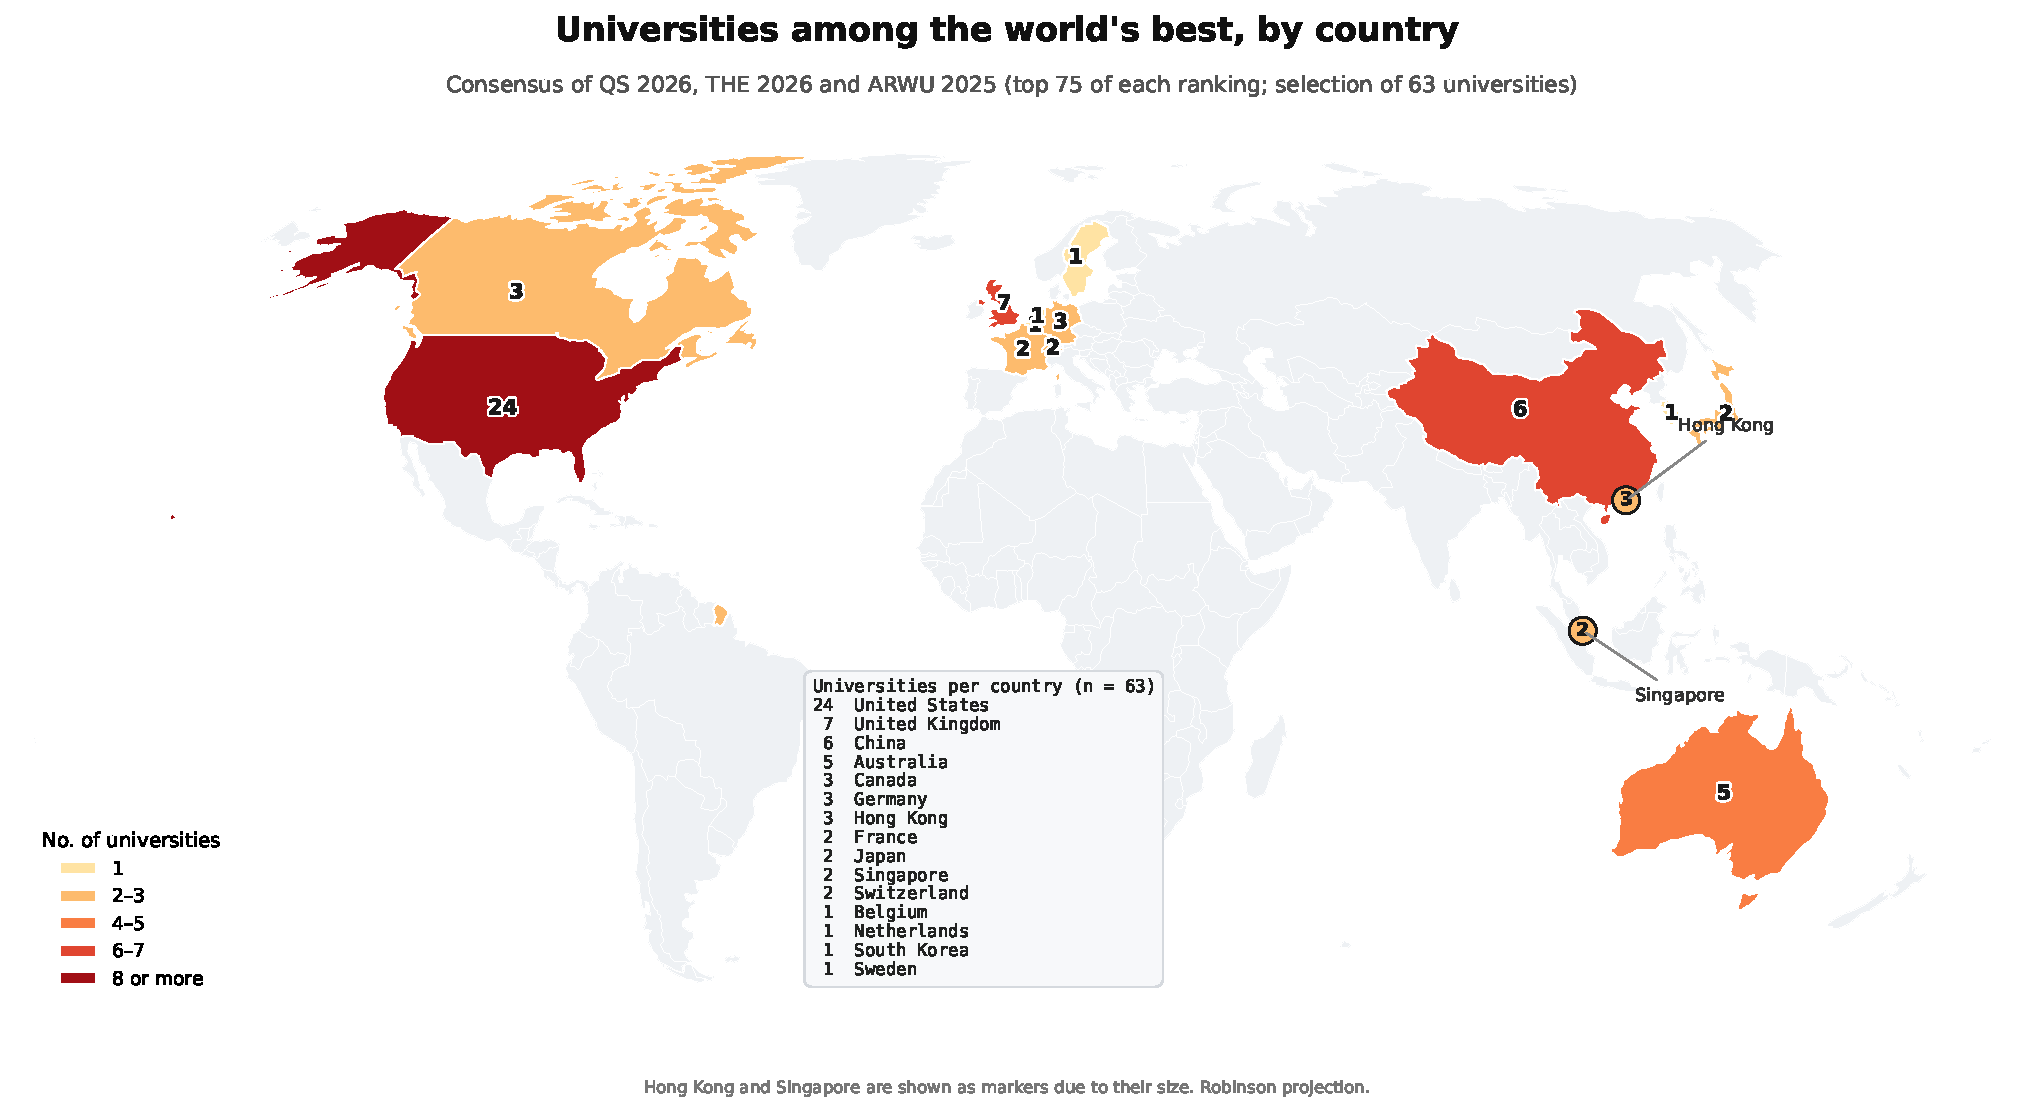
\includegraphics[width=\textwidth]{mapa_calor_paises.pdf}
	\caption{Distribution by country of the 63 universities selected by consensus of QS~2026, THE~2026 and ARWU~2025. Colour intensity indicates the number of universities per country; Hong~Kong and Singapore are shown as markers given their small size on the map.}\label{fig:mapa-paises}
\end{figure}

Each site was reviewed in August 2026 with the study's five dimensions. Only one required adjustment. As the LOPDP applies only in Ecuador \citep{lopdp2021,reglamentolopdp2023}, elsewhere we checked whether the institution cites the framework applicable in its jurisdiction: in Europe, the GDPR \citep{gdpr2016}, the British data-protection law \citep{ukdpa2018}, the \emph{ePrivacy} rules \citep{eprivacy2002} and the Swiss federal act \citep{fadp_ch}; in the United States, the CCPA \citep{ccpa2018}, FERPA \citep{ferpa1974} and HIPAA \citep{hipaa1996}; in China, the PIPL \citep{pipl2021}; in Japan, the APPI \citep{appi2003}; in Singapore, the PDPA \citep{pdpa2012}; in South Korea, the PIPA \citep{pipa2011}; in Australia, the \emph{Privacy Act} \citep{privacyact1988}; in Canada, the FIPPA or Quebec's law \citep{fippa_on,quebec_privacy}; and in Hong~Kong, the PDPO \citep{pdpo_hk}. Figure~\ref{fig:lineas-leyes} orders these frameworks chronologically by their year of implementation.

\begin{figure}[H]
	\centering
	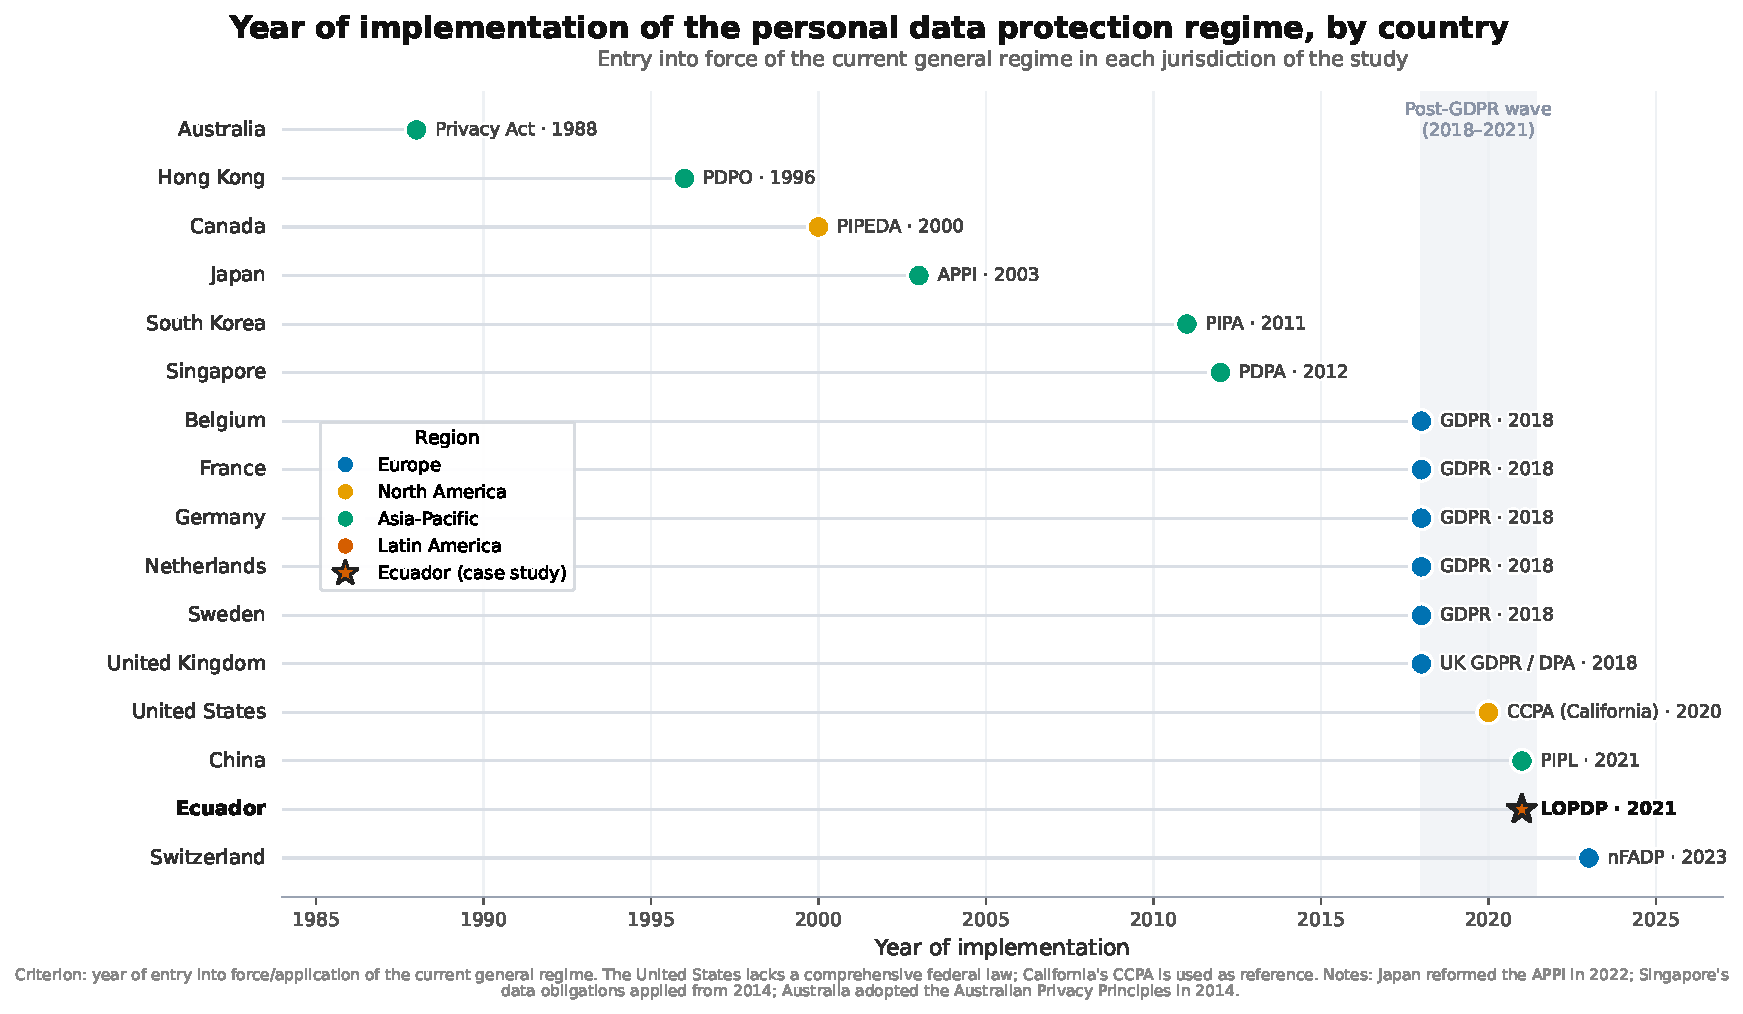
\includegraphics[width=\textwidth]{linea_tiempo_leyes.pdf}
	\caption{Year of implementation of the general personal-data protection regime in each jurisdiction of the study. The entry into force or application of the current regime is used; the United States lacks a comprehensive federal law, so California's CCPA is used as reference. Ecuador is highlighted as the case study.}\label{fig:lineas-leyes}
\end{figure}

That chronology helps situate the Ecuadorian case. The arc runs from 1988, when Australia passed its \emph{Privacy Act}, to 2023, with the revised Swiss law, and reveals two clusters: a slow diffusion through the 2000s and 2010s, and a jump in 2018, when the GDPR's application aligned the whole European bloc ---and, by extension, the United Kingdom--- in a single year. Ecuador (LOPDP, 2021) belongs to the latest wave, alongside China (PIPL, 2021) and California (CCPA, 2020), so its framework is among the most recent in the set; that regulatory youth helps explain ---though it does not excuse--- why its translation to the public web is still incipient, and serves as a backdrop for the differences examined below.

The other four dimensions were kept intact so the contrast would be legitimate, but two of them ---cookies and accessibility--- were additionally subjected to a live automated audit, because the documentary method does not execute JavaScript and underestimates both banners and the barriers that appear only on the rendered page. In August 2026 each of the 126 sites was visited with a real browser ---Chromium driven by Playwright--- over a connection in Ecuador, in a single reproducible pass with a read-only script. Before interacting with any banner, the pre-consent state was recorded: the number and names of the cookies, which of them were tracking cookies (analytics and marketing), the consent-management platform (CMP) signature and the presence of a banner. On the same load the axe-core~4.13 engine was injected and conformance with the Web Content Accessibility Guidelines was assessed \citep{wcag21}, assigning each violation its criterion, its principle ---perceivable, operable, understandable or robust--- and its conformance level (A, AA or AAA).

The scope of this measurement deserves a note. An automated tool demonstrates non-conformance ---a single failure breaks a level--- but does not certify full conformance, since a large share of the criteria requires human review and no tool covers the guidelines in full \citep{fischer2025coverage}; axe's results therefore cover the machine-testable subset, which at each site was accompanied by the number of checks the tool itself flags for manual review. For cookies, measuring from a single vantage point has a deliberate consequence: sites subject to the GDPR neither show their banner nor block tracking for a visitor outside the European Union, so what is observed is exactly what an Ecuadorian user experiences, not what a European would see.

\section{Results}\label{sec:resultados}
Table~\ref{tab:comp} sets both sets side by side, indicator by indicator. Table~\ref{tab:reg} breaks the world group down by region, and the appendices hold the detail for each institution: Appendix~\ref{ap:mundo} (Table~\ref{tab:mundo}) for the 63 in the world and Appendix~\ref{ap:ecuador} (Table~\ref{tab:ecuador}) for the 63 in Ecuador.

\begin{table}[htbp]
	\centering
	\caption{Data privacy on the websites: 63 best universities in the world vs.\ 63 Ecuadorian HEIs.}\label{tab:comp}
	\small
	\begin{tabular}{@{}p{7.2cm}cccc@{}}
		\toprule
		\textbf{Indicator} & \textbf{World} & \textbf{World \%} & \textbf{Ecuador} & \textbf{Ecuador \%} \\
		\midrule
	Privacy policy / treatment notice & 58/63 & 92.1\% & 39/63 & 61.9\% \\
	Applicable legal framework cited (LOPDP in Ecuador) & 48/63 & 76.2\% & 31/63 & 49.2\% \\
	Data subject's rights listed & 47/63 & 74.6\% & 35/63 & 55.6\% \\
	Data protection officer (DPO) or contact & 54/63 & 85.7\% & 24/63 & 38.1\% \\
	Tracking before consent (live) & 43/63 & 68.3\% & 40/63 & 63.5\% \\
	Active consent manager (CMP, live) & 12/63 & 19.0\% & 14/63 & 22.2\% \\
	Accessibility / affirmative action (declared) & 47/63 & 74.6\% & 7/63 & 11.1\% \\
	WCAG conformance: reaches level A (live) & 25/63 & 39.7\% & 5/63 & 7.9\% \\
	Valid TLS certificate & 63/63 & 100.0\% & 58/63 & 92.1\% \\
		\bottomrule
	\end{tabular}
	\par\vspace{2pt}
	\footnotesize\RaggedRight\textit{Note:} both censuses $n=63$. Rows marked \emph{live} come from the real-browser audit (August 2026, axe-core 4.13) described in the methods; the rest, from the documentary review. ``Reaches level~A'' means the site shows no automatic level-A failures, the machine-testable subset of WCAG conformance.
\end{table}

\subsection{Treatment notice, legal framework and rights}
The widest gap does not appear in the technical details but in the foundations. Nine out of ten universities in the world reference publish a privacy policy; in Ecuador six out of ten do. If that policy is also required to name the legal framework that underpins it, the world drops to 76.2\% and Ecuador to 49.2\%. The gap becomes an abyss at the point that matters most to whoever uses the site: knowing whom to address. A data-protection officer or a specific channel appears at 85.7\% of the world's best and at barely 38.1\% of the Ecuadorian ones, and the enumeration of the data subject's rights repeats the bias, 74.6\% against 55.6\%. As these figures come from documents read without any rendering, the contrast is firm: Ecuador lacks not so much the paper as the legal depth of that paper and an open channel to exercise the rights it states.

None of this makes the reference a paragon. Harvard, Michigan or Washington University in St.~Louis do not enumerate rights or cite a framework in their main notice, and two major Chinese universities, Fudan and Shanghai Jiao Tong, do not even publish a central policy on their institutional portal. That institutions of such standing carry such gaps is a reminder that academic prestige does not guarantee data care, and confirms that compliance can be more appearance than substance \citep{munot2025compliance}.

\subsection{Cookie use}
The static method could not see the banners or the cookies injected by JavaScript, so this dimension was checked live, visiting each site in a real browser and recording, before any consent, which cookies were placed, which consent-management platform (CMP) loaded and whether a banner appeared. Figure~\ref{fig:cookies-live} summarises the contrast and belies the naive reading that a scarce banner means little tracking.

\begin{figure}[H]
	\centering
	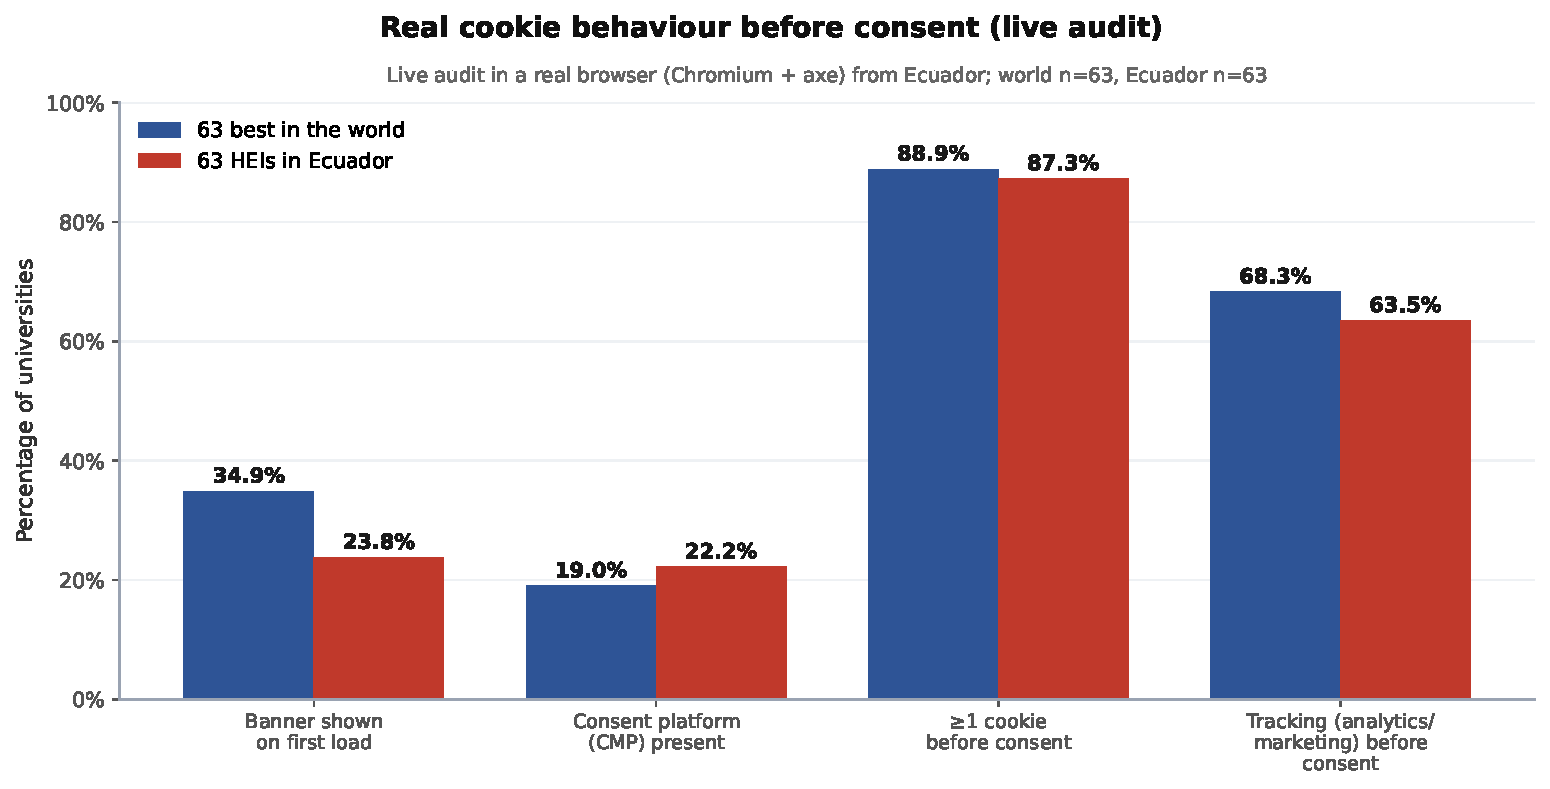
\includegraphics[width=\textwidth]{fig_cookies_live.pdf}
	\caption{Live check of cookie behaviour before consent: 63 best universities in the world vs.\ the 63 Ecuadorian HEIs (world $n=63$; Ecuador $n=63$). At each site the state prior to any interaction with the banner was read.}\label{fig:cookies-live}
\end{figure}

The visible banner is a minority on both sides (34.9\% in the world, 23.8\% in Ecuador), but that snapshot deceives, because many European sites show it only to visitors from the European Union and this audit was run from Ecuador. What is telling lies in the cookies placed \emph{without} any consent, and there is no gap: in Ecuador 87.3\% place at least one and 63.5\% load tracking cookies ---analytics or marketing: Google Analytics and Ads, the Meta pixel, TikTok, Microsoft Clarity or Hotjar---; in the world's best those figures are, if anything, slightly higher: 88.9\% and 68.3\%. Seen from an Ecuadorian user's browser, the world elite tracks before consent as much as the country's universities, or a little more.

That result forces a comfortable intuition to be corrected. The restraint usually attributed to universities subject to the GDPR does not protect those who visit them from outside the European Union: for an Ecuadorian user no banner appears and nothing is blocked, and tracking fires all the same. The ``consent theatre'' ---interfaces that nudge acceptance and disguise refusal, or cookie managers that do not actually block--- is thus not a local defect but a global phenomenon, and the presence of a CMP, somewhat more common in Ecuador (22.2\%) than in the world (19.0\%), does not change the outcome. It is precisely what the measurement literature described after the GDPR, when notices multiplied without treatment improving: the mere presence of a banner does not guarantee valid consent \citep{degeling2019value,kretschmer2021cookie,nouwens2020dark,gray2021dark,habib2022okay}.

\subsection{Affirmative action, inclusion and security}
The other deep crack is accessibility, taken here as a vehicle for inclusion. Three out of four elite universities offer an accessibility statement or tools; in Ecuador one in nine does. Behind that difference lie concrete legal obligations, such as the \emph{Americans with Disabilities Act} \citep{ada1990} and Section~508 of the \emph{Rehabilitation Act} \citep{section508} in the United States or the \emph{European Accessibility Act} \citep{eaa2019} in the European Union, and on the Ecuadorian side an almost non-existent practice in the portals, a lag regional research has documented for years \citep{campoverdemolina2023accessibility,acostavargas2020dataset}. On communications encryption the story is kinder: valid HTTPS covers 100\% of the world group and 92.1\% of the Ecuadorian one, where five institutions carry faulty certificates.

\begin{table}[htbp]
	\centering
	\caption{World group by region: privacy policy, legal framework cited, DPO and accessibility (HEIs complying out of the regional total).}\label{tab:reg}
	\small
	\begin{tabular}{@{}lccccc@{}}
		\toprule
		\textbf{Region} & \textbf{n} & \textbf{Privacy} & \textbf{Legal fr.} & \textbf{DPO} & \textbf{Access.} \\
		\midrule
	USA & 24 & 24 & 18 & 23 & 22 \\
	United Kingdom & 7 & 6 & 4 & 5 & 7 \\
	Cont.\ Europe & 10 & 10 & 9 & 10 & 8 \\
	China & 6 & 2 & 2 & 3 & 0 \\
	Hong Kong & 3 & 3 & 3 & 2 & 3 \\
	Asia (others) & 5 & 5 & 4 & 4 & 0 \\
	Australia & 5 & 5 & 5 & 4 & 4 \\
	Canada & 3 & 3 & 3 & 3 & 3 \\
		\bottomrule
	\end{tabular}
\end{table}

The regional breakdown dismantles the idea of a homogeneous ``developed world''. Continental Europe leads on citing the legal framework, with nine of its ten universities naming the GDPR and its national transposition; the United States leads on accessibility, with 22 of 24 portals, pushed by the ADA; and Hong~Kong's three houses comply without flaw under the PDPO. China is the group's exception: only two of its six universities name a legal framework and none publishes an accessibility statement. The moral is that topping world research and caring for privacy on the web are distinct matters, which do not always travel together.

\subsection{Measured WCAG conformance}
The declared accessibility in Table~\ref{tab:comp} only says whether the institution promises inclusion; to know whether it delivers, each portal was audited with axe-core, checking its code against the WCAG criteria. Table~\ref{tab:wcag} summarises the result and Figure~\ref{fig:wcag-niveles} shows its most telling feature.

\begin{table}[htbp]
	\centering
	\caption{WCAG conformance measured live (axe-core): 63 best in the world vs.\ 63 Ecuadorian HEIs. Percentage of sites unless stated.}\label{tab:wcag}
	\small
	\begin{tabular}{@{}p{8.4cm}cc@{}}
		\toprule
		\textbf{Indicator (live audit)} & \textbf{World} & \textbf{Ecuador} \\
		\midrule
	Median WCAG violations per site & 2 & 4 \\
	Sites with no automatic failure & 9.5\% & 0.0\% \\
	Sites reaching level A & 39.7\% & 7.9\% \\
	Links without accessible name (2.4.4, level A) & 23.8\% & 81.0\% \\
	Insufficient contrast (1.4.3, level AA) & 25.4\% & 79.4\% \\
	Images without text alternative (1.1.1, level A) & 15.9\% & 30.2\% \\
	Level where failures concentrate & AAA & A \\
		\bottomrule
	\end{tabular}
\end{table}

\begin{figure}[H]
	\centering
	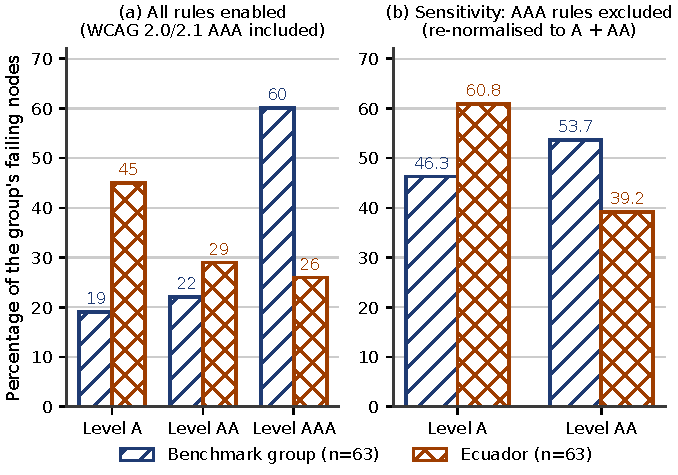
\includegraphics[width=\textwidth]{fig_wcag_niveles.pdf}
	\caption{Distribution of WCAG failing nodes by conformance level (percentage of each group's total; axe-core, August 2026). Ecuador concentrates its failures at level~A ---the basic tier---, whereas the world's best do so at level~AAA ---the excellence tier.}\label{fig:wcag-niveles}
\end{figure}

The figures belie any complacency on both sides: no Ecuadorian university ---and only 9.5\% of the world's best--- passes the audit without a single automatic failure, and the median number of violations per site is four in Ecuador against two in the world. But the decisive difference lies not in quantity but in severity. In the world reference, 60\% of the failing nodes belong to level~AAA ---the excellence tier, above all enhanced contrast---, and barely 19\% fall at level~A; in Ecuador the proportion is reversed and 45\% of the failures hit that level~A, the most basic. Put differently, the world stumbles chasing excellence and Ecuador stumbles at the threshold. The most eloquent case is criterion 2.4.4, which asks that every link have text a screen reader can announce: 81.0\% of Ecuadorian sites breach it against 23.8\% in the world. The most affected principle in both groups is the perceivable one, through colour contrast, but in Ecuador an operable deficit ---links and controls--- is added that in the reference is marginal; these are, moreover, the same error types that dominate WCAG audits of other public portals \citep{iniesto2025service}.

Bringing the two live audits together reveals a finding that transcends the ranking: the quality of accessibility and respect for privacy do not go hand in hand. Across the 126 universities, the correlation between the volume of accessibility failures and the number of tracking cookies is practically nil (Spearman $\rho=0.04$). Caring for one does not predict caring for the other: in Ecuador, one in three institutions limits tracking but fails basic accessibility, and barely 3\% achieve both; in the world, 30\% are accessible at level~A yet still track without permission. They are, therefore, two independent ethical commitments ---accessibility and privacy---, each with its own legal lever and its own inertia, and no university, in the country or on the planet, has resolved both at once.

\section{Discussion}\label{sec:discusion}
The comparison orders the Ecuadorian system's priorities. What is pressing is neither the infrastructure, with HTTPS already near-universal, nor the cookie banner, an elusive indicator of dubious quality even among the leaders. What is pressing is governance: a policy anchored in the law, rights written with clarity and, above all, a data controller one can write to and a portal anyone can use. That elite universities meet these points so often is no spontaneous merit but a response to laws that impose them, from the GDPR's duty to name an officer to the ADA's accessibility mandates. The LOPDP and its regulation enclose equivalent requirements, still barely visible in the institutions' public window.

The reference, even so, counsels against idealising. Having a policy does not prove good treatment; the banners of the most reputed universities often breach the conditions of free consent \citep{nouwens2020dark,gray2021dark}; and even top-tier names show hard-to-justify gaps. The sensible goal for Ecuador is not to copy those institutions' façade, but to reach what their façade sometimes hides and what the law already demands: respectful treatment of its community's data.

The live data adds a nuance that corrects the easy reading. On paper Ecuador lags, but in the real behaviour of cookies there is no such gap: its universities track the user before asking permission almost as much as the world's best (63.5\% against 68.3\%), and the latter, seen from outside the European Union, do not behave better. The ``consent theatre'' is a shared problem, not an Ecuadorian singularity; and since the GDPR's protection stops at the community border, the student who consults a European university's portal from Ecuador is as exposed as on their own institution's. The lesson for Ecuador is therefore not that it tracks more than anyone, but that the solution will not come from imitating a restraint the reference applies only indoors.

\section{Conclusions}\label{sec:conclusiones}
Measured against the 63 best universities in the world, the Ecuadorian system shows wide gaps precisely where people's trust is most at stake: policies anchored in the law (61.9\% against 92.1\%) and a data-protection officer or channel (38.1\% against 85.7\%). To these is added accessibility, where the live audit reveals that no institution is free of failures, but that Ecuador breaches basic-level criteria ---81\% of its sites have links without an accessible name--- while the world only stumbles at the excellence tier. That is the order in which to act. The live check, by contrast, tempers the cookie front: two out of three Ecuadorian HEIs track the user before asking permission, but the world's best do so to the same degree for a non-European visitor, so the problem is global and not a national failing. Publishing a policy that expressly invokes the LOPDP and its regulation, giving a data controller a name and an email address, making portals accessible according to the WCAG guidelines \citep{wcag21} ---starting with the basics--- and requiring cookie managers to actually block would suffice to close most of the distance. A challenge remains that Ecuador shares with Cambridge or MIT and that no front-page statistic resolves: that what is promised on the page is truly honoured in the treatment.

\begin{appendices}
\section{Appendices}
The appendices gather the institution-by-institution evidence underpinning this work's figures, so the count can be redone and individual cases audited. Appendix~\ref{ap:mundo} lists the 63 universities in the world (Table~\ref{tab:mundo}) and Appendix~\ref{ap:ecuador} the 63 Ecuadorian institutions (Table~\ref{tab:ecuador}). In both, each row is an official website and each column one of the assessed dimensions, with the same marker legend; the columns do not fully match between the two because the legal framework was adapted to each jurisdiction and because transparency (LOTAIP) applies only to the Ecuadorian case. Exact addresses and consultation dates appear in the data matrices accompanying this work.

\section{Matrix of the 63 best universities in the world}\label{ap:mundo}
Legend: \si~complies; \no~absent or non-compliant; \textbf{P}~partial (limited scope or generic framework); \nd~not detectable (dynamic content). Rankings: QS 2026, THE 2026 and ARWU 2025 (position; ``--'' means outside that ranking's top~75). Country in ISO code. Columns: Pol.\ (privacy policy), Frame (legal framework cited), Rights, DPO, Cook.\ (cookie policy), Acc.\ (accessibility).

\footnotesize
\begin{longtable}{@{}r l c c c c c c c c c c@{}}
	\caption{Data privacy matrix of the 63 best universities in the world.}\label{tab:mundo}\\
	\toprule
	\textbf{\#} & \textbf{Abbr.} & \textbf{C} & \textbf{QS} & \textbf{THE} & \textbf{ARWU} & \textbf{Pol.} & \textbf{Frame} & \textbf{Rights} & \textbf{DPO} & \textbf{Cook.} & \textbf{Acc.} \\
	\midrule
	\endfirsthead
	\multicolumn{12}{c}{\textit{(Table~\ref{tab:mundo}, continued)}}\\
	\toprule
	\textbf{\#} & \textbf{Abbr.} & \textbf{C} & \textbf{QS} & \textbf{THE} & \textbf{ARWU} & \textbf{Pol.} & \textbf{Frame} & \textbf{Rights} & \textbf{DPO} & \textbf{Cook.} & \textbf{Acc.} \\
	\midrule
	\endhead
	\midrule
	\multicolumn{12}{r}{\textit{Continued on next page}}\\
	\endfoot
	\bottomrule
	\endlastfoot
1 & MIT & US & 1 & 2 & 3 & \si & \si & \si & \si & \no & \si \\
	2 & Stanford & US & 3 & 5 & 2 & \si & \si & \si & \si & \si & \si \\
	3 & Harvard & US & 5 & 5 & 1 & \si & \si & \no & \no & \no & \si \\
	4 & Oxford & UK & 4 & 1 & 6 & \si & \si & \si & \si & \si & \si \\
	5 & Cambridge & UK & 6 & 3 & 4 & \no & \pc & \no & \no & \si & \si \\
	6 & Caltech & US & 10 & 7 & 9 & \si & \si & \no & \si & \no & \si \\
	7 & UC Berkeley & US & 17 & 9 & 5 & \si & \si & \no & \si & \no & \si \\
	8 & Princeton & US & 25 & 3 & 7 & \si & \si & \si & \si & \no & \si \\
	9 & Imperial & UK & 2 & 8 & 26 & \si & \si & \pc & \no & \si & \si \\
	10 & U Chicago & US & 13 & 15 & 10 & \si & \pc & \si & \si & \no & \no \\
	11 & ETH Zurich & CH & 7 & 11 & 22 & \si & \si & \si & \si & \no & \si \\
	12 & Yale & US & 21 & 10 & 11 & \si & \si & \pc & \si & \no & \si \\
	13 & UPenn & US & 15 & 14 & 14 & \si & \pc & \si & \si & \no & \si \\
	14 & UCL & UK & 9 & 22 & 14 & \si & \pc & \si & \si & \si & \si \\
	15 & Cornell & US & 16 & 18 & 12 & \si & \pc & \si & \si & \no & \si \\
	16 & Tsinghua & CN & 17 & 12 & 18 & \si & \si & \si & \si & \no & \no \\
	17 & Peking & CN & 14 & 13 & 23 & \pc & \pc & \no & \no & \no & \no \\
	18 & Johns Hopkins & US & 24 & 16 & 19 & \si & \si & \si & \si & \no & \si \\
	19 & Columbia & US & 38 & 20 & 8 & \si & \si & \si & \si & \si & \si \\
	20 & Toronto & CA & 29 & 21 & 25 & \si & \si & \si & \si & \no & \si \\
	21 & UCLA & US & 46 & 18 & 16 & \si & \si & \si & \si & \no & \si \\
	22 & NUS & SG & 8 & 17 & 56 & \si & \si & \si & \si & \no & \no \\
	23 & U Tokyo & JP & 36 & 26 & 31 & \si & \si & \si & \no & \no & \no \\
	24 & TUM & DE & 22 & 27 & 45 & \si & \si & \si & \si & \no & \no \\
	25 & Melbourne & AU & 19 & 37 & 38 & \si & \si & \si & \si & \no & \no \\
	26 & Edinburgh & UK & 34 & 29 & 37 & \si & \si & \si & \si & \no & \si \\
	27 & EPFL & CH & 22 & 35 & 44 & \si & \si & \si & \si & \no & \si \\
	28 & Michigan & US & 45 & 23 & 33 & \si & \no & \no & \si & \no & \no \\
	29 & Northwestern & US & 42 & 30 & 31 & \si & \pc & \si & \si & \si & \si \\
	30 & Fudan & CN & 30 & 36 & 41 & \no & \no & \no & \no & \no & \no \\
	31 & PSL & FR & 28 & 48 & 34 & \si & \si & \si & \si & \no & \no \\
	32 & HKU & HK & 11 & 33 & 67 & \si & \si & \si & \si & \no & \si \\
	33 & Zhejiang & CN & 49 & 39 & 24 & \si & \pc & \si & \si & \no & \no \\
	34 & NYU & US & 55 & 31 & 28 & \si & \si & \si & \si & \no & \si \\
	35 & SJTU & CN & 47 & 40 & 30 & \no & \no & \no & \no & \no & \no \\
	36 & KCL & UK & 31 & 38 & 61 & \si & \pc & \si & \si & \si & \si \\
	37 & UCSD & US & 66 & 47 & 20 & \si & \si & \si & \si & \no & \si \\
	38 & LMU & DE & 58 & 34 & 42 & \si & \si & \si & \si & \no & \si \\
	39 & Duke & US & 62 & 28 & 46 & \si & \si & \si & \si & \no & \si \\
	40 & Manchester & UK & 35 & 56 & 46 & \si & \si & \pc & \si & \no & \si \\
	41 & UBC & CA & 40 & 45 & 53 & \si & \si & \pc & \si & \no & \si \\
	42 & Sydney & AU & 25 & 53 & 72 & \si & \si & \si & \si & \no & \si \\
	43 & Paris-Saclay & FR & 70 & 68 & 13 & \si & \si & \si & \si & \si & \si \\
	44 & Kyoto & JP & 57 & 61 & 46 & \si & \pc & \si & \si & \no & \no \\
	45 & Illinois & US & 70 & 41 & 53 & \si & \si & \si & \si & \no & \si \\
	46 & UT Austin & US & 68 & 50 & 49 & \si & \si & \si & \si & \no & \si \\
	47 & UW & US & -- & 25 & 17 & \si & \si & \si & \si & \no & \si \\
	48 & NTU & SG & 12 & 31 & -- & \si & \si & \si & \si & \no & \no \\
	49 & McGill & CA & 27 & 41 & -- & \si & \si & \si & \si & \si & \si \\
	50 & CUHK & HK & 32 & 41 & -- & \si & \si & \si & \no & \no & \si \\
	51 & CMU & US & 52 & 24 & -- & \si & \si & \si & \si & \no & \si \\
	52 & Wisconsin & US & -- & 53 & 36 & \si & \si & \no & \si & \si & \si \\
	53 & USTC & CN & -- & 51 & 40 & \pc & \si & \si & \si & \no & \no \\
	54 & WUSTL & US & -- & 67 & 26 & \si & \no & \no & \si & \no & \si \\
	55 & Monash & AU & 36 & 58 & -- & \si & \si & \no & \no & \no & \si \\
	56 & SNU & KR & 38 & 58 & -- & \si & \si & \si & \si & \no & \no \\
	57 & Heidelberg & DE & -- & 49 & 51 & \si & \si & \si & \si & \no & \si \\
	58 & HKUST & HK & 44 & 58 & -- & \si & \si & \si & \si & \no & \si \\
	59 & Karolinska & SE & -- & 53 & 50 & \si & \pc & \si & \si & \si & \si \\
	60 & TU Delft & NL & 47 & 57 & -- & \si & \si & \si & \si & \si & \si \\
	61 & ANU & AU & 32 & 73 & -- & \si & \si & \pc & \si & \no & \si \\
	62 & KU Leuven & BE & 60 & 46 & -- & \si & \si & \si & \si & \si & \si \\
	63 & Queensland & AU & 42 & -- & 65 & \si & \si & \si & \si & \no & \si \\
\end{longtable}
\normalsize

\section{Matrix of the 63 Ecuadorian HEIs (SENESCYT/CES)}\label{ap:ecuador}
Legend: \si~complies; \no~absent or non-compliant; \textbf{P}~partial (limited scope, e.g.\ only postgraduate, admissions or mobile app); \nv~not verifiable by the method (blocked site or non-machine-readable document); \nd~not detectable (dynamic content). Type: P (public), C (co-financed), A (self-financed). Columns: Pol.\ (privacy policy), LOPDP (explicit mention of the law), Rights, DPO, Cook.\ (cookie banner), Incl.\ (accessibility/inclusion), Transp.\ (transparency/LOTAIP).

\footnotesize
\begin{longtable}{@{}r l c c c c c c c c@{}}
	\caption{Data privacy matrix of the 63 Ecuadorian HEIs.}\label{tab:ecuador}\\
	\toprule
	\textbf{\#} & \textbf{Abbr.} & \textbf{Type} & \textbf{Pol.} & \textbf{LOPDP} & \textbf{Rights} & \textbf{DPO} & \textbf{Cook.} & \textbf{Incl.} & \textbf{Transp.} \\
	\midrule
	\endfirsthead
	\multicolumn{10}{c}{\textit{(Table~\ref{tab:ecuador}, continued)}}\\
	\toprule
	\textbf{\#} & \textbf{Abbr.} & \textbf{Type} & \textbf{Pol.} & \textbf{LOPDP} & \textbf{Rights} & \textbf{DPO} & \textbf{Cook.} & \textbf{Incl.} & \textbf{Transp.} \\
	\midrule
	\endhead
	\midrule
	\multicolumn{10}{r}{\textit{Continued on next page}}\\
	\endfoot
	\bottomrule
	\endlastfoot
1 & EPN & P & \si & \si & \si & \no & \nd & \no & \si \\
	2 & ESPOL & P & \si & \si & \si & \si & \nd & \no & \si \\
	3 & ESPOCH & P & \no & \no & \no & \no & \nd & \no & \si \\
	4 & ESPAM MFL & P & \no & \no & \no & \no & \nd & \no & \si \\
	5 & ESPE & P & \si & \si & \si & \si & \nd & \si & \si \\
	6 & UCE & P & \nv & \no & \no & \no & \nd & \no & \si \\
	7 & UCuenca & P & \si & \si & \si & \no & \si & \no & \si \\
	8 & UG & P & \si & \si & \si & \si & \nd & \no & \si \\
	9 & UNL & P & \no & \no & \no & \no & \nd & \no & \si \\
	10 & UAE & P & \no & \no & \no & \no & \nd & \no & \si \\
	11 & UTA & P & \si & \nv & \nv & \nv & \nd & \nv & \si \\
	12 & UTB & P & \si & \si & \si & \si & \nd & \no & \si \\
	13 & UTC & P & \si & \no & \no & \no & \nd & \no & \nd \\
	14 & UTMACH & P & \si & \si & \si & \si & \nd & \no & \si \\
	15 & UTM & P & \no & \no & \no & \no & \nd & \no & \si \\
	16 & UTN & P & \pc & \si & \si & \no & \nd & \no & \si \\
	17 & UTEQ & P & \pc & \si & \no & \no & \nd & \no & \si \\
	18 & UTELVT & P & \no & \no & \no & \no & \nd & \no & \si \\
	19 & UEB & P & \si & \nv & \nv & \nv & \nd & \si & \si \\
	20 & UNESUM & P & \pc & \nv & \no & \no & \nd & \no & \si \\
	21 & UNEMI & P & \si & \si & \si & \no & \nd & \no & \si \\
	22 & UEA & P & \si & \no & \si & \no & \nd & \no & \si \\
	23 & UPSE & P & \pc & \si & \si & \si & \nd & \pc & \si \\
	24 & ULEAM & P & \no & \no & \no & \no & \nd & \no & \si \\
	25 & UNACH & P & \si & \si & \si & \si & \nd & \si & \si \\
	26 & UNAE & P & \no & \no & \no & \no & \nd & \no & \si \\
	27 & UPEC & P & \no & \pc & \no & \no & \nd & \no & \si \\
	28 & Yachay Tech & P & \no & \no & \no & \no & \nd & \no & \si \\
	29 & Ikiam & P & \si & \si & \si & \si & \nd & \no & \si \\
	30 & UArtes & P & \si & \si & \si & \si & \nd & \no & \si \\
	31 & Amawtay Wasi & P & \no & \no & \no & \no & \nd & \no & \si \\
	32 & USECIPOL & P & \pc & \no & \no & \no & \nd & \no & \si \\
	33 & IAEN & P & \si & \si & \si & \no & \si & \si & \si \\
	34 & UASB & P & \si & \si & \si & \si & \nd & \no & \si \\
	35 & FLACSO & P & \no & \no & \no & \no & \nd & \no & \si \\
	36 & PUCE & C & \si & \si & \si & \si & \nd & \no & \si \\
	37 & UCSG & C & \si & \si & \si & \si & \si & \no & \si \\
	38 & UCACUE & C & \si & \si & \si & \si & \nd & \si & \si \\
	39 & ULVR & C & \no & \no & \no & \no & \nd & \no & \si \\
	40 & UTPL & C & \si & \si & \si & \si & \nd & \no & \nd \\
	41 & UTE & C & \si & \no & \no & \no & \nd & \si & \nd \\
	42 & UDA & C & \no & \no & \no & \no & \nd & \no & \si \\
	43 & UPS & C & \si & \si & \si & \no & \nd & \no & \si \\
	44 & UISEK & A & \si & \no & \si & \no & \nd & \no & \no \\
	45 & UEES & A & \si & \si & \si & \si & \nd & \no & \no \\
	46 & USFQ & A & \si & \si & \si & \si & \nd & \no & \no \\
	47 & UDLA & A & \si & \si & \si & \si & \nd & \no & \no \\
	48 & UIDE & A & \si & \si & \si & \si & \nd & \no & \si \\
	49 & UNIANDES & A & \si & \no & \si & \no & \nd & \no & \no \\
	50 & UPACÍFICO & A & \nv & \no & \no & \no & \nd & \no & \no \\
	51 & UTI & A & \si & \no & \si & \no & \nd & \no & \si \\
	52 & Casa Grande & A & \si & \si & \si & \si & \nd & \no & \no \\
	53 & UTEG & A & \si & \si & \si & \si & \nd & \no & \si \\
	54 & UISRAEL & A & \si & \nv & \nv & \nv & \nd & \nv & \nv \\
	55 & UDET & A & \no & \no & \no & \no & \nd & \no & \no \\
	56 & UMET & A & \si & \nv & \nv & \nv & \nd & \no & \si \\
	57 & U. Otavalo & A & \nv & \nv & \no & \no & \nd & \no & \nv \\
	58 & USGP & A & \si & \si & \si & \si & \nd & \no & \si \\
	59 & U. Hemisferios & A & \si & \si & \si & \si & \si & \no & \si \\
	60 & UNIB.E & A & \si & \no & \si & \no & \nd & \no & \no \\
	61 & ECOTEC & A & \si & \si & \si & \si & \si & \no & \si \\
	62 & UDR & A & \no & \no & \no & \no & \nd & \no & \no \\
	63 & UBE & A & \si & \si & \si & \si & \si & \si & \no \\
\end{longtable}
\normalsize
\end{appendices}

\bibliography{references}

\end{document}
